
\documentclass[unknownkeysallowed]{beamer}
\usetheme{Madrid}
\usepackage{subfig}
\usepackage{xcolor}
\title{Dimensionality reduction with UMAP}
\subtitle{Advanced Data Mining seminar}
\author{Jakub Bartczuk}
\centering
\date{March 2020}
\begin{document}
\maketitle

\begin{frame}{Overview}
\tableofcontents[section,subsection]
\end{frame}

\begin{frame}{Teaser}
\framesubtitle{Reducing dimensionality of COIL20 Dataset}
\begin{figure}[ht]\centering\begin{minipage}[b]{0.45\linewidth}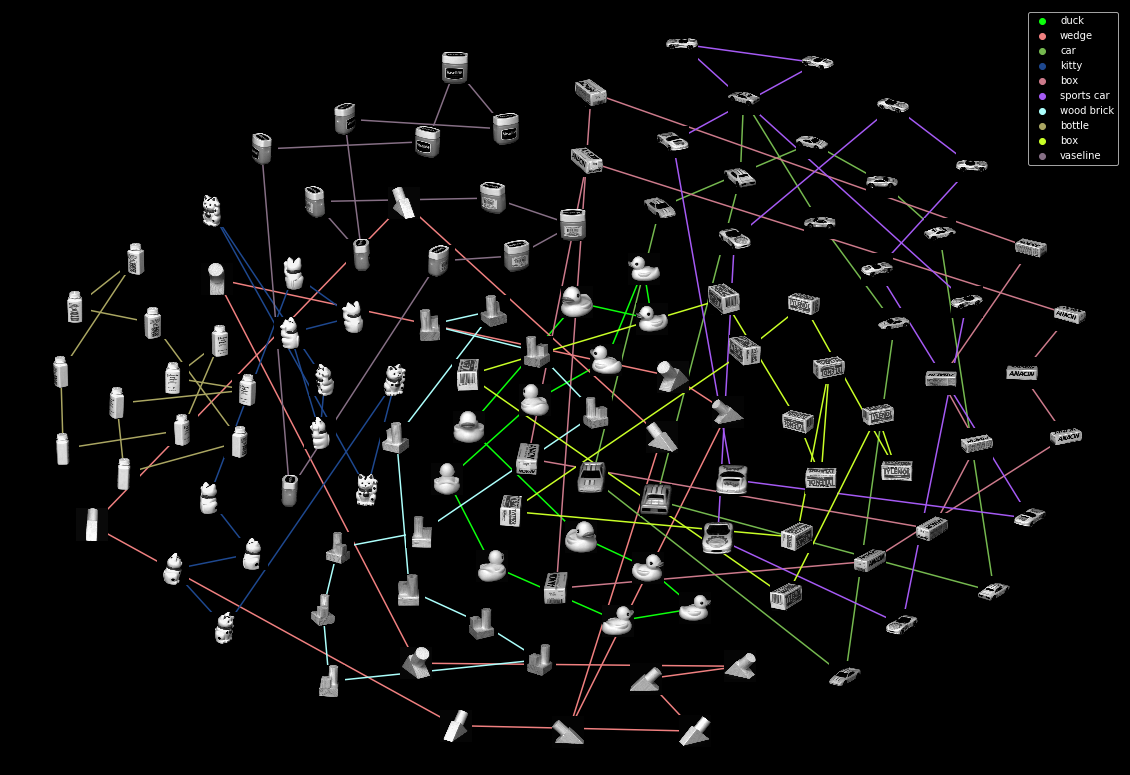
\includegraphics[width=\textwidth]{coil_tsne.png}\caption{tSNE}\label{fig:minipage1}\end{minipage}\quad\begin{minipage}[b]{0.45\linewidth}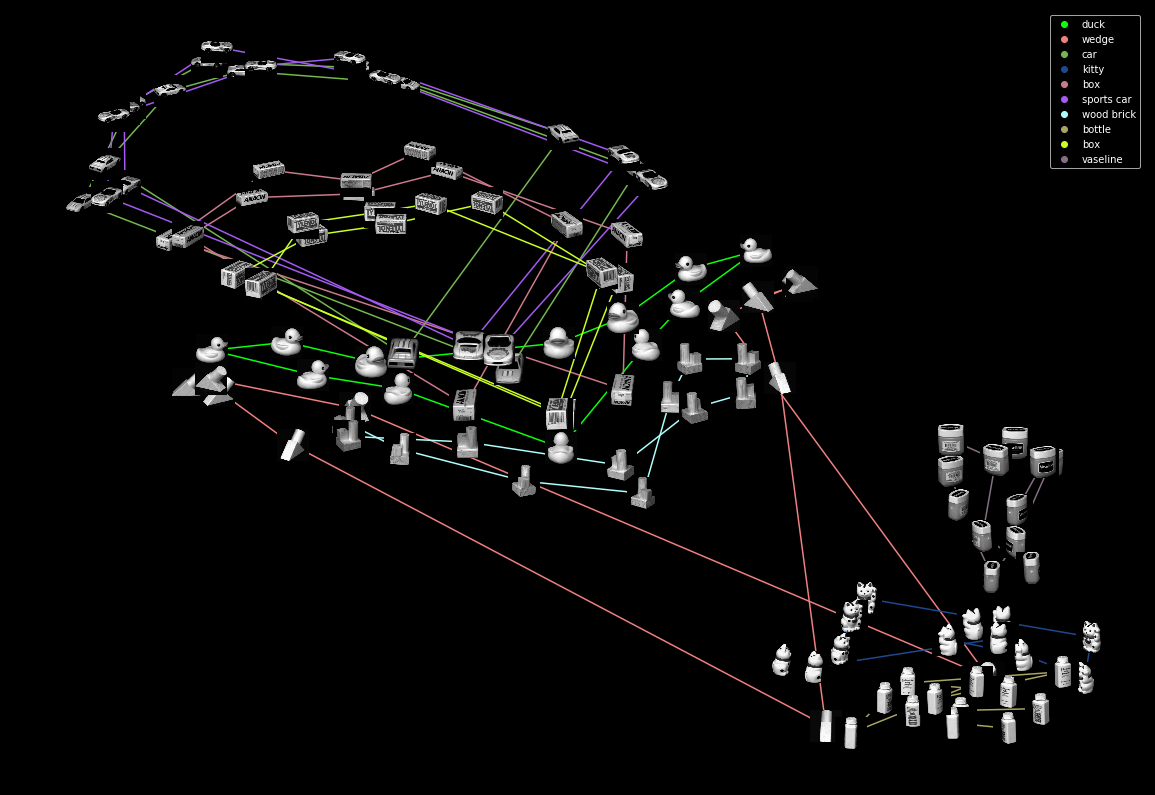
\includegraphics[width=\textwidth]{coil_umap.png}\caption{UMAP}\label{fig:minipage2}\end{minipage}\end{figure}
\end{frame}

\section{Manifold learning recap}
\begin{frame}{Manifold learning recap}

\begin{itemize}
\item We want to uncover lower-dimensional structure in high-dimensional space
\item Is the structure linear? If yes, use PCA
\item What to do if it is not linear?
\end{itemize}
\end{frame}
\begin{frame}{Manifold learning recap}



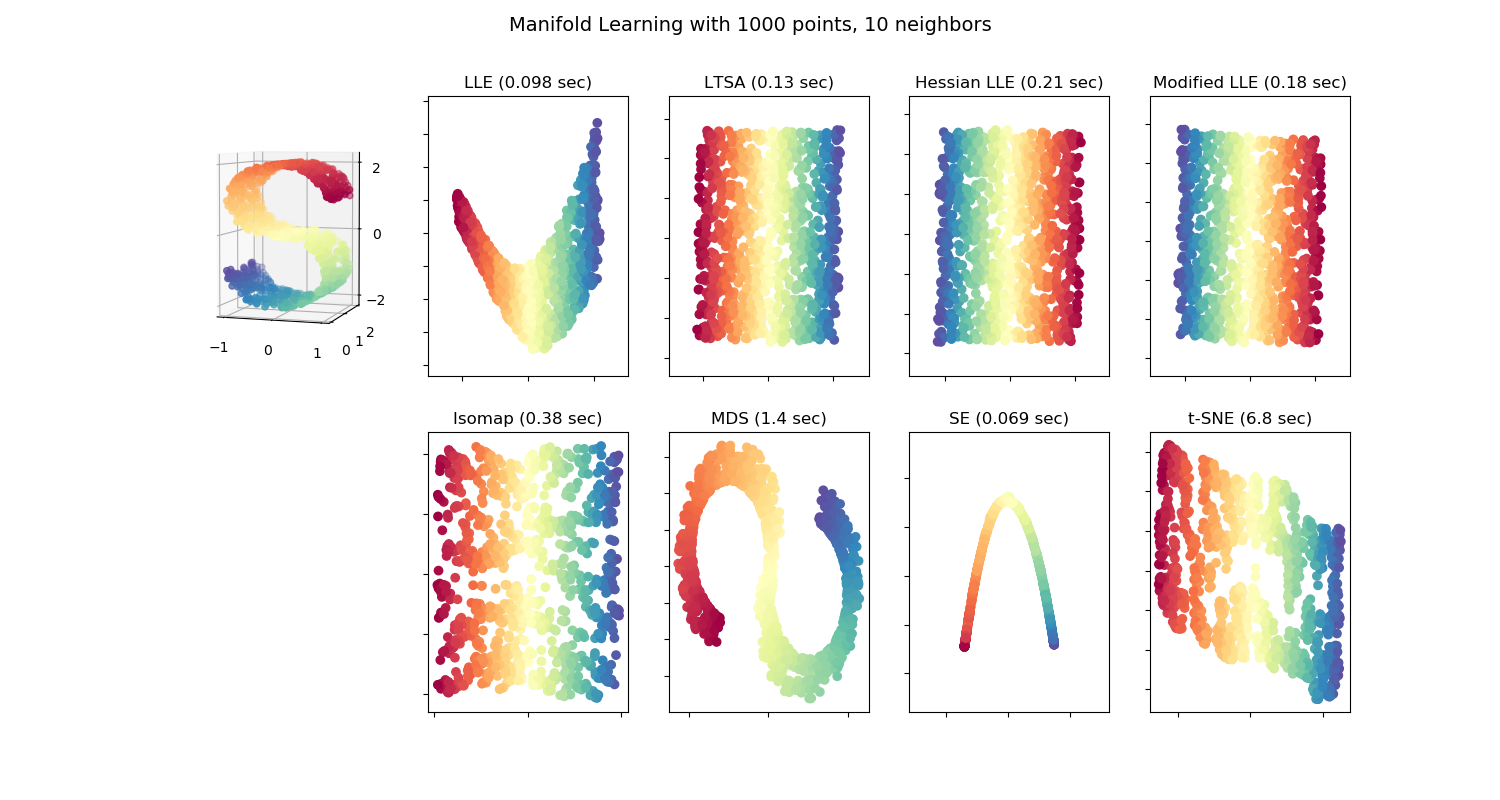
\includegraphics[width=\textwidth,height=0.8\textheight,keepaspectratio]{manifold_algorithms}

\end{frame}

\subsection{Multidimensional Scaling}
\begin{frame}{Classical Multidimensional Scaling}


$$D_{i,j} = \|x_i - x_j\|^2$$

Find $y$'s, $D'_{i,j} = \|y_i - y_j\|^2$ 

Such that $D' \approx D$

\end{frame}


\begin{frame}{Classical MDS properties}

\begin{itemize}
    \item easy to compute - decompose low-rank matrix from D
    \item fast - Euclidean distance matrix just couple of vectorized matrix computations
    \item treats all distortions alike
\end{itemize}



\begin{block}{What structure does MDS preserve?}
The last property basically means that we preserve local and global structure alike.

\begin{itemize}
    \item $x$'s are close - they are close in embedding.
    \item $x$'s are distant - they are equally distant in embedding.
\end{itemize}

\end{block}
\end{frame}
\subsection{Distances, graphs and matrix decomposition}

\begin{frame}{Distances, graphs and matrix decomposition}

\begin{block}{Why we may not care about preserving exact large distances in embedding space}
\end{block}

Idea: Calculate distance along manifold

\end{frame}

\begin{frame}{MDS breakdown}


\begin{enumerate}
   \item estimate distances between some pairs of close points
   \item make graph $(X, E)$ with edges weighted by distance
   \item define $D$ as distance from graph
   \item decompose matrix that represents the graph
\end{enumerate}{}

\begin{block}{Getting manifold learning algorithms from schematic}

\begin{itemize}
    \item Setting $E = \{((x_i, x_j), \|x_i - x_j\|^2) | x_i, x_j \in X \}$ (complete graph) we get classical MDS
    \item Modifying steps 1-3 will get us Isomap, Hessian Eigenmaps
    \item tSNE and UMAP will change step 4
\end{itemize}
\end{block}



\end{frame}

\section{Stochastic Neighbor Embedding}
\begin{frame}{Stochastic Neighbor Embedding}

Idea: embed into lower-dimensional space, preserve distance statistics

$$q_{j|i} = \frac{\textcolor{blue}{f}(\|y_i - y_j\|)}{\sum_{k \neq j}\textcolor{blue}{f}(\|y_i - y_k\|)}, p_{j|i} = \frac{exp(-\|x_i - x_j\|^2 / \textcolor{red}{\sigma^2_i})}{\sum_{k \neq j}exp(-\|x_i - x_k\|^2/\textcolor{red}{\sigma^2_i})}$$

$$KL(p, q) = \sum_{i, j} p_{j|i} log\frac{p_{j|i}}{q_{j|i}}$$

\begin{block}{Notes}
Choice of $\textcolor{blue}{f}$ determines algorithm:
\begin{itemize}
    \item $\textcolor{blue}{f(x) = exp(-x^2)}$ - original SNE
    \item $\textcolor{blue}{f(x) = (1 + x^2)^{-1}}$ - tSNE (note this is density of Cauchy distribution up to a constant)
\end{itemize}
\end{block}
\end{frame}

\begin{frame}{Stochastic Neighbor Embedding}

\begin{block}{Perplexity}
\textcolor{red}{$\sigma_i$} gives rise to perplexity $P_i = 2^{H(p_i)}$ which controls effective neighborhood size at $x_i$.
\end{block}

\begin{block}{Algorithm}
\begin{itemize}
	\item for each $x_i$ find $\sigma_i$ that matches given perplexity
    \item initialize $y_i$ randomly
    \item minimize KL with gradient descent w.r.t. $y_i$
\end{itemize}
\end{block}

\end{frame}


\begin{frame}{Problems with SNE}

\begin{block}{Crowding problem}
Somewhat fixed by using t Distribution which has longer tails (not so concentrated about maximum)
\end{block}

\begin{block}{Complexity}
?? Trees
\end{block}

\end{frame}

\section{UMAP}


\begin{frame}{ELI5 UMAP}

\end{frame}

\subsection{Topological preliminaries}


\begin{frame}{Topological preliminaries}

\end{frame}

\section{Experiments}

\begin{frame}{Experiments}

\end{frame}

\section{Practicalities}
\begin{frame}{Python implementations}

	\begin{block}{tSNE and other algorithms}
		\begin{itemize}
			\item scikit-learn implements tSNE, MDS, Isomap, Hessian Eigenmaps, Locally Linear Embedding
			\item faster implementations available in \texttt{megaman} package
		\end{itemize}
	\end{block}
	
	\begin{block}{UMAP}
		\begin{itemize}
			\item original author's package (\texttt{pip install umap-learn})
			\item GPU accelerated NVidia \texttt{rapids (cuML)} 
		\end{itemize}
	\end{block}
\end{frame}
\end{document}
